%Author: Siddhesh Wani
%Date: December 9, 2015




\documentclass[12pt]{article}
\usepackage{tikz}
\usetikzlibrary{shapes.geometric, arrows}
\usepackage{hyperref}
\usepackage[a4paper]{geometry}
%DO NOT EDIT start
%Define different shapes to be used in flowchart
\tikzstyle{startstop} = [rectangle, rounded corners, minimum width=3cm, minimum height=1cm,text centered, draw=black, fill=red!30]
\tikzstyle{io} = [trapezium, trapezium left angle=70, trapezium right angle=110, minimum width=3cm, minimum height=1cm, text centered, draw=black, fill=blue!30]
\tikzstyle{process} = [rectangle, minimum width=3cm, minimum height=1cm, text centered, draw=black, fill=orange!30]
\tikzstyle{decision} = [diamond, minimum width=3cm, minimum height=1cm, text centered, draw=black, fill=green!30]
\tikzstyle{arrow} = [thick,->,>=stealth]
\tikzstyle{connector} = [signal,draw=black,fill=olive!30]%,text width=1cm,text height=1.5cm,align=center]
%DO NOT EDIT end




\begin{document}
\newgeometry{top=1cm, bottom=0.5cm,right=1cm,left=1.5cm}

\vspace*{2cm}
\begin{center}

\section*{\hypertarget{initSCI2C}INIT\_SCI2C.sci}
{Siddhesh Wani}\\
 
\end{center}


\textbf{Introduction}\\
`INIT\_SCI2C' initialises sscilab2c extension using the given input parameters. 'FileInfo' and `SharedInfo' structures are initialised and stored in .dat files. Directory 
structure is created. Other few .dat files required by extension are initialised and saved on disk. \\

\begin{center}
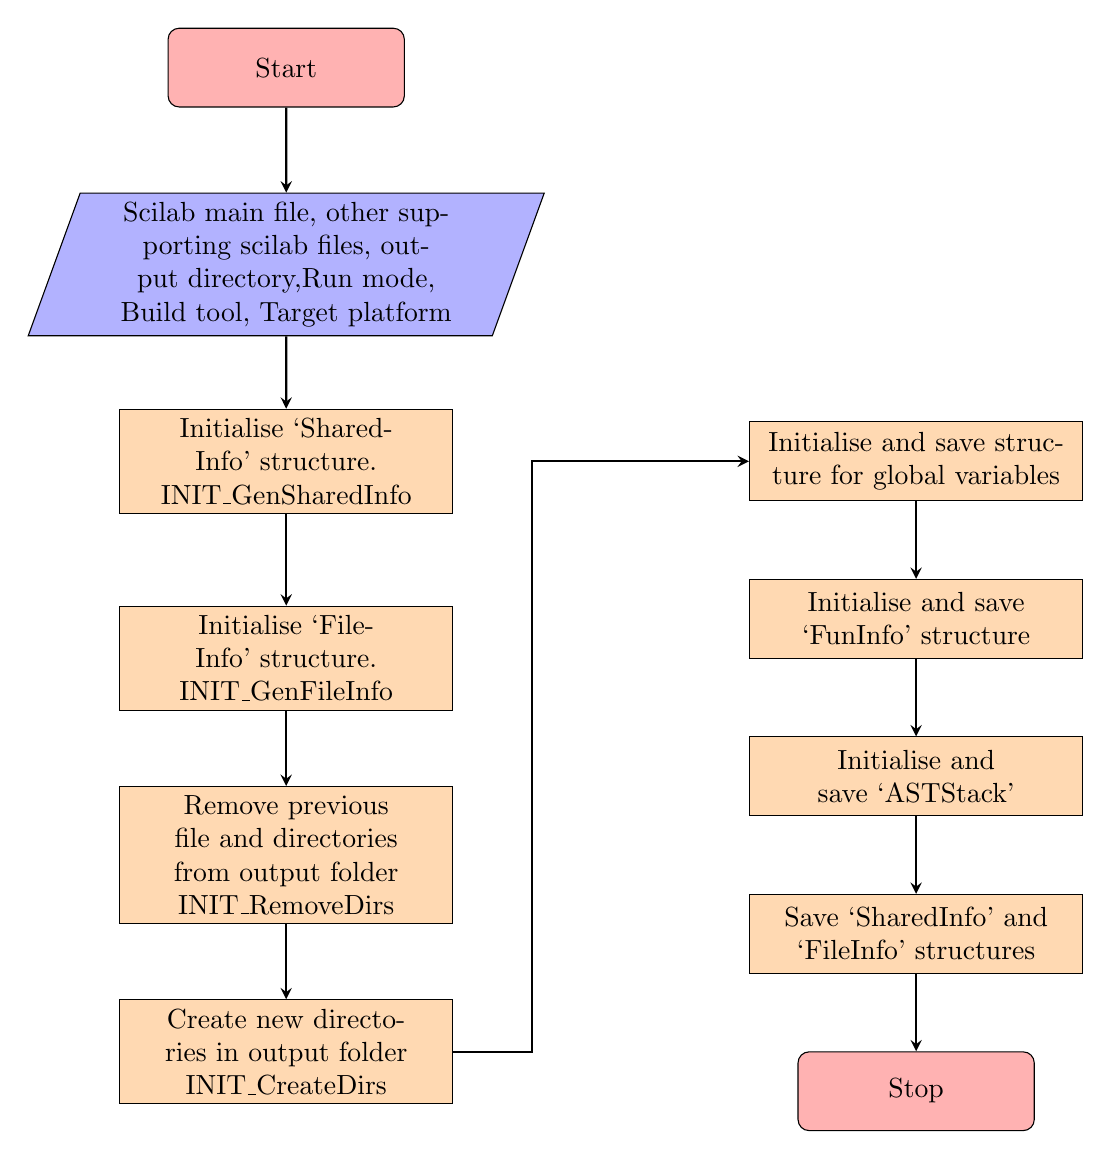
\begin{tikzpicture}[node distance=2cm]
\node (start) [startstop] {Start};
\node (input)[io, below of=start, text width=5cm, yshift=-0.5cm] {Scilab main file, other supporting scilab files, output directory,Run mode, Build tool, Target platform};
\node (sharedinfo)[process, below of=input,text width=4cm, yshift=-0.5cm]{Initialise `SharedInfo' structure. \\ INIT\_GenSharedInfo};
\node (fileinfo)[process, below of=sharedinfo,text width=4cm, yshift=-0.5cm]{Initialise `FileInfo' structure. \\ INIT\_GenFileInfo};
\node (remove)[process, below of=fileinfo,text width=4cm, yshift=-0.5cm]{Remove previous file and directories from output folder \\ INIT\_RemoveDirs};
\node (create)[process, below of=remove,text width=4cm, yshift=-0.5cm]{Create new directories in output folder \\ INIT\_CreateDirs};
\node (global)[process, right of=sharedinfo,text width=4cm,xshift=6cm]{Initialise and save structure for global variables};
\node (funinfo)[process, below of=global,text width=4cm]{Initialise and save `FunInfo' structure};
\node (aststack)[process, below of=funinfo,text width=4cm]{Initialise and save `ASTStack'};
\node (save)[process, below of=aststack,text width=4cm]{Save `SharedInfo' and `FileInfo' structures};
\node (stop) [startstop, below of=save]{Stop};


\draw [arrow] (start) -- (input);
\draw [arrow] (input) -- (sharedinfo);
\draw [arrow] (sharedinfo) -- (fileinfo);
\draw [arrow] (fileinfo) -- (remove);
\draw [arrow] (remove) -- (create);
\draw [arrow] (create.east) --++ (1cm,0) |- (global);
\draw [arrow] (global) -- (funinfo);
\draw [arrow] (funinfo) -- (aststack);
\draw [arrow] (aststack) -- (save);
\draw [arrow] (save) -- (stop);

\end{tikzpicture}
\end{center}

\end{document}